% !TEX TS-program = pdflatex
% !TEX encoding = UTF-8 Unicode

% This is a simple template for a LaTeX document using the "article" class.
% See "book", "report", "letter" for other types of document.

\documentclass[11pt]{article} % use larger type; default would be 10pt

\usepackage[utf8]{inputenc} % set input encoding (not needed with XeLaTeX)

%%% Examples of Article customizations
% These packages are optional, depending whether you want the features they provide.
% See the LaTeX Companion or other references for full information.

%%% PAGE DIMENSIONS
\usepackage{geometry} % to change the page dimensions
\geometry{a4paper} % or letterpaper (US) or a5paper or....
% \geometry{margin=2in} % for example, change the margins to 2 inches all round
% \geometry{landscape} % set up the page for landscape
%   read geometry.pdf for detailed page layout information

\usepackage{graphicx} % support the \includegraphics command and options

% \usepackage[parfill]{parskip} % Activate to begin paragraphs with an empty line rather than an indent

%%% PACKAGES
\usepackage{booktabs} % for much better looking tables
\usepackage{array} % for better arrays (eg matrices) in maths
\usepackage{paralist} % very flexible & customisable lists (eg. enumerate/itemize, etc.)
\usepackage{verbatim} % adds environment for commenting out blocks of text & for better verbatim
\usepackage{subfig} % make it possible to include more than one captioned figure/table in a single float
% These packages are all incorporated in the memoir class to one degree or another...

%%% HEADERS & FOOTERS
\usepackage{fancyhdr} % This should be set AFTER setting up the page geometry
\pagestyle{fancy} % options: empty , plain , fancy
\renewcommand{\headrulewidth}{0pt} % customise the layout...
\lhead{}\chead{}\rhead{}
\lfoot{}\cfoot{\thepage}\rfoot{}

%%% SECTION TITLE APPEARANCE
\usepackage{sectsty}
\allsectionsfont{\sffamily\mdseries\upshape} % (See the fntguide.pdf for font help)
% (This matches ConTeXt defaults)

%%% ToC (table of contents) APPEARANCE
\usepackage[nottoc,notlof,notlot]{tocbibind} % Put the bibliography in the ToC
\usepackage[titles,subfigure]{tocloft} % Alter the style of the Table of Contents
\renewcommand{\cftsecfont}{\rmfamily\mdseries\upshape}
\renewcommand{\cftsecpagefont}{\rmfamily\mdseries\upshape} % No bold!

%%% END Article customizations

%%% The "real" document content comes below...

\title{Brief Article}
\author{Author one\and Author two\and Author three}
%\date{} % Activate to display a given date or no date (if empty),
         % otherwise the current date is printed 

\begin{document}
\maketitle

\begin{abstract}
When using hardware description languages(HDL) to do circuit design, we need to handle much unnecessary details, like the wire connections and timing. And different implementations of an algorithm are vary in time and gate resources. The  desinger have to rewrite the code and put much effort on considering the sequential signals if he/she wants to gain optimations on time or resource usement. So in this work, we desiged some new HDL syntex that the desinger can use to express the reconfigurable part of the circut. we also implement a Verilog compiler to handle the new syntex and dig out all the possible trade-offs between time and spcace of the design, generate Verilog codes depends on the designer's choices during the interactive compiling process.\newline\newline
\textbf{Key words: }IP core, HDL, configuration, sequential circuit
\end{abstract}



\section{Introduction}

\begin{figure}
\centering
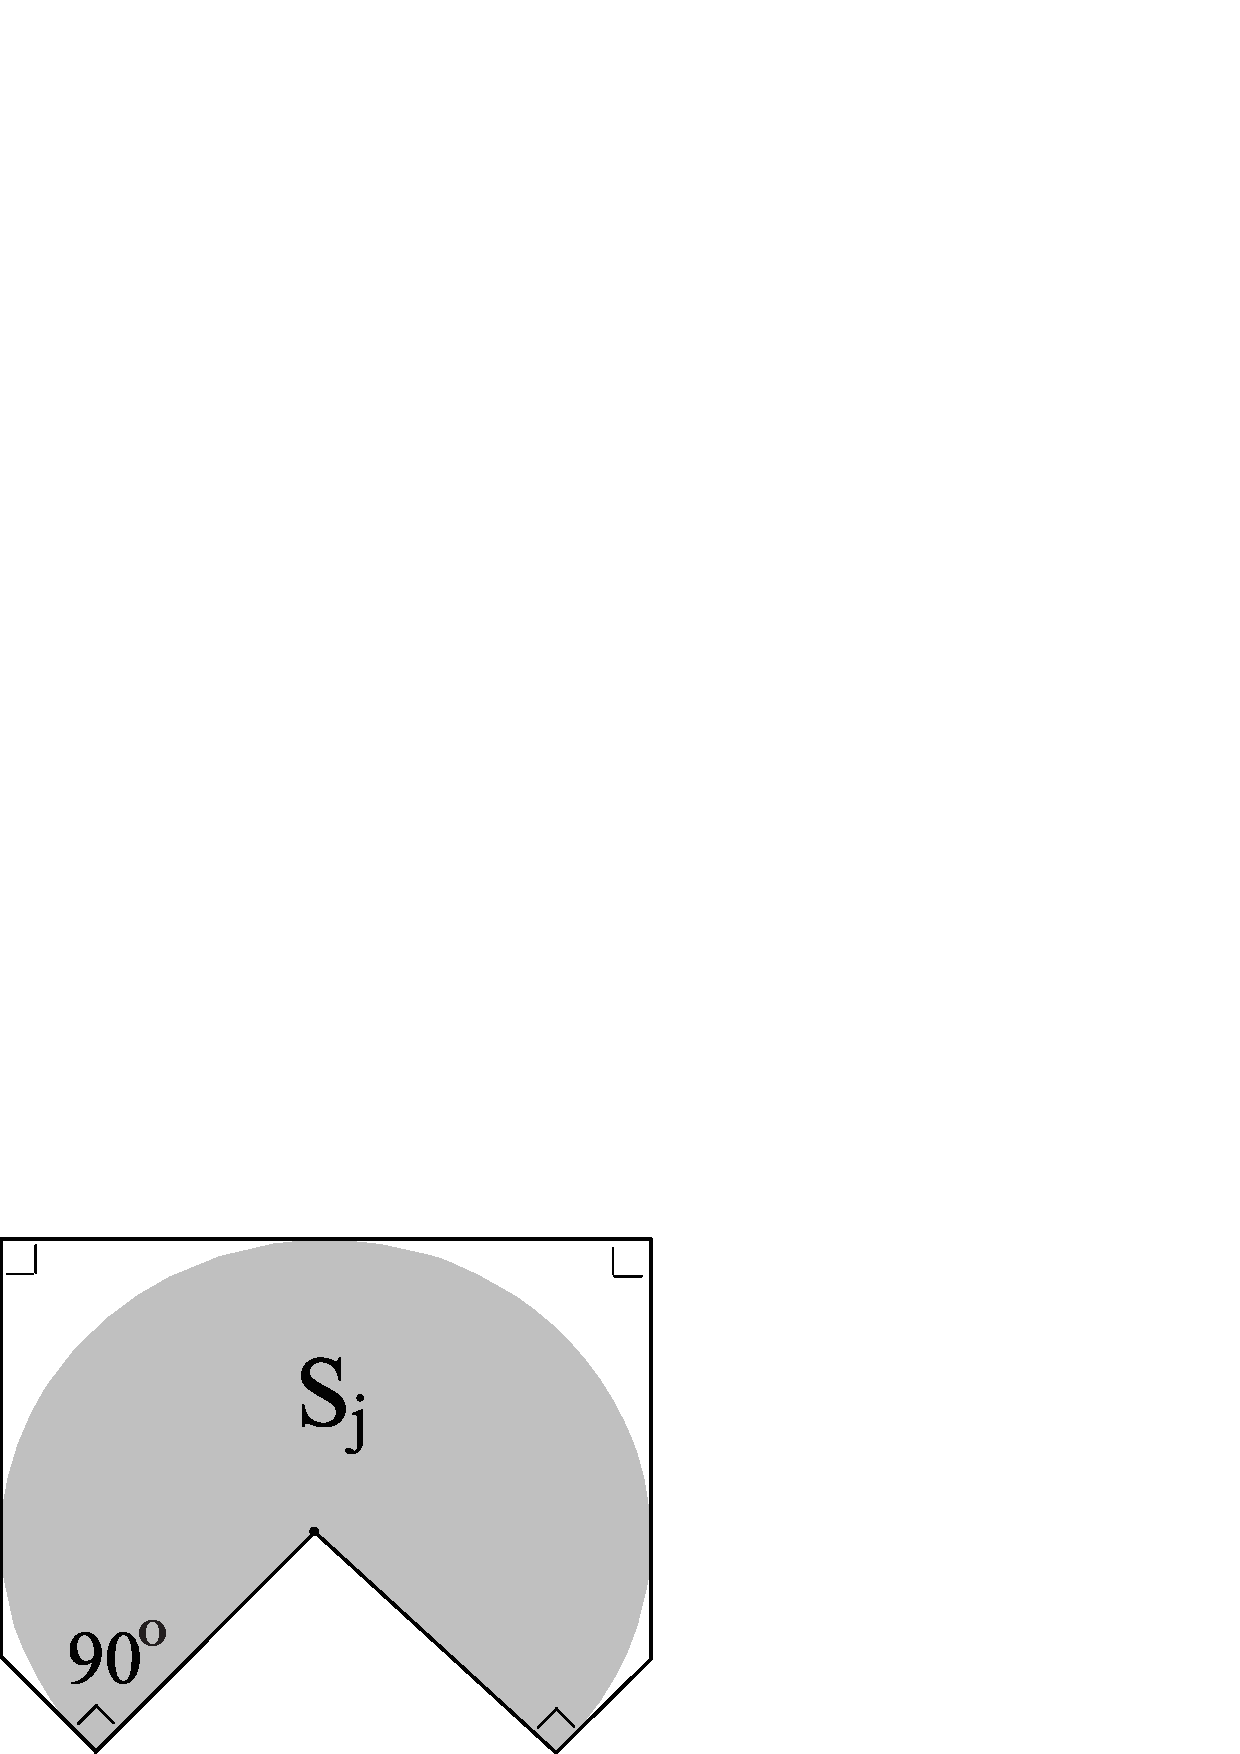
\includegraphics{fig10a}
\caption{Example of Enlarged Polygon}
\label{fig:10}
\end{figure}

\subsection{State the problem}
Hardware description language(HDL) based IP synthesis has been the industry standard in recen years. However they are still very low level in expressing a digital circuit. Take an example from Verilog, when designing a calculator to compute the following mathematic expression using sequential circuit, we need to divide the mathmatical expression into tiny steps and figure out the operations in each step.\newline
 \begin{math}y = 5 * 2^{x_1} + 5 * 2^{x_2} + 5 * 2^{x_3} + 5 * 2^{x_4} \end{math} \newline
They are diffrent kinds of computing methods, here are two:\newline
METHOD 1: \newline
STEP1: Calculate \begin{math}5 * 2^{x_1}\end{math}, \begin{math}5 * 2^{x_2}\end{math}, \begin{math}5 * 2^{x_3}\end{math}, \begin{math}5 * 2^{x_3}\end{math}, \begin{math}5 * 2^{x_4}\end{math} separately and store the temporary results.\newline
STEP2: Do the addtions of the temporary results.\newline \newline
METHOD2: \newline
STEP1: Initialize the summation.\newline
STEP2: Calculate \begin{math} 5 * 2^{x_1}\end{math}\newline
STEP3: Add the multiply result to summation, make a partial summation.\newline
STEP4: Calculate \begin{math} 5 * 2^{x_2}\end{math}\newline
STEP5: Add the multiply result to summation.\newline
\dots \newline 
STEP9: Add the multiply result to summation. \newline\newline
We can see that METHOD1 and METHOD2 have different numbers of steps in the calculation, however the resource costs are also different. In METHOD1 it need four shifters to do the multiply,four regs to hold the multiply results  in STEP1, and three adders in STEP2. On the other side, METHOD2 just needs one shifter, one reg and one adder, since STEP2, STEP4, STEP6 and STEP8 can share the same shifter, as well as STEP3, STEP5, STEP7 use the same adder.\newline
Their implementation are vary very much in details in Verilog code.(backup using code example?) \newline
So in order to free designers from detail things and dig out all the possible implementing methods, we need to express this kind of circuit in higher level and point out the different configurations in compiling time.\newline\newline
\subsection{State your contributions}
In our work,we proposed some functional languagae-like syntax that can be used to describle reconfigurable structures in circuits and can be embeded with traditional Verilog code. We implemented a parser to pick up the novel statements and defined optimization rules to translate these statements into tranditional Verilog codes depends on the designer's optimazation choice. An interactive compiling system was implemented, designer can model circuit in mathematical expression level and get trad-offs between time and space easily(just by interacting with the compiler). A scoring function was designed to compute the time and space cost for different optimize rules.\newline\newline 

\section{The problem}
\subsection{calculation unit reuse}
Example from DCT,FFT
\subsection{circuit block reuse and it's timing cost}
Example:sbox in AES
\subsection{Not easy to modify a design to gain time-space trade off}
wire connections, control signals and orgnization of reused resources, all these make a lot changes of the source code
\section{Our idea}
SV+ program $\rightarrow$ SV+ compiler $\rightarrow$ Verilog code
\section{Details and implementation}
\subsection{new syntax}
map,fold,forloop. How to use them and when to use them.
\subsection{translation rules and scoring function}
\section{Experiments}
1. Code is shorter. \newline
2. Different time and resource cost of the entire circuit by different optimization  choices.\newline
3. 
\section{Related work}
1. High level synthesis\newline
2. Code generater, spiral\newline
3. Functional languages in hardware design
\end{document}
